\documentclass{article}
\usepackage{analemma,times}
\input{math_commands.tex}
\usepackage{hyperref}
\usepackage{url}
\usepackage{graphicx}
\usepackage{subfigure}
\usepackage{booktabs}
\usepackage{adjustbox}
\usepackage{amsmath}
\usepackage{amssymb}
\usepackage{mathtools}
\usepackage{amsthm}
\usepackage{multirow}
\usepackage{color}
\usepackage{colortbl}
\usepackage{array}
\usepackage[capitalize,noabbrev]{cleveref}
\usepackage{xspace}
\graphicspath{{figures/}}

\title{From Incidents to Replayable Exploits:\\An Empirical Study of DeFi Attack Surfaces}
\author{}
\analemmafinalcopy

\begin{document}
\maketitle
\fancyhead{}
\renewcommand{\headrulewidth}{0pt}
\pagestyle{fancy}
\thispagestyle{fancy}

\begin{abstract}
Public DeFi hack reporting is abundant, but research claims about exploitability often collapse together corpus statistics, protocol-specific reasoning, and proof-of-concept replay results. This paper rebuilds that pipeline explicitly. Using a normalized corpus of 2{,}036 public incidents, including 1{,}378 DeFi-labeled cases, we combine three evidence layers already present in the repository: a broad incident corpus, five deep protocol audits with 87 manually triaged findings, and a 24-protocol pure on-chain verification study augmented by replay engineering for representative historical exploits. The resulting picture is narrower than raw incident volume implies. In the verified protocol set, only one protocol exhibits a high-confidence pure on-chain exploit path, while three additional cases are conditional or integration-dependent, yielding an exposure ratio of approximately 16.7\%. The replay batch further shows that only 3 of 12 shortlisted incidents have been converted into concrete replay logic so far, for a replay conversion rate of 25\%. These results support a methodological claim: DeFi security research should be framed as an incident-to-replay workflow, not as a flat list of hacks or scanner findings. We conclude with a conservative but actionable interpretation of which exploit families remain most replayable and what evidence is still missing for stronger claims.
\end{abstract}

\section{Introduction}
\label{sec:introduction}

Decentralized finance has generated a large public archive of incidents, exploit writeups, protocol post-mortems, and security dashboards, yet those artifacts rarely line up into a single evidentiary chain. Corpus-wide datasets are broad but noisy; protocol audits are deep but local; exploit proofs of concept are concrete but narrow. As a result, DeFi security discourse often shifts between incompatible units of analysis without explicitly stating when the underlying evidence has changed. A repository may contain hundreds of scanner findings, a dashboard may report thousands of incidents, and a post-mortem may present a single elegant exploit path, but none of those views alone answers a central research question: which publicly reported incidents correspond to replayable pure on-chain exploit mechanisms rather than operational compromise, social engineering, or context-specific failures?

This paper addresses that gap using the artifact set that already exists in the repository. The repository contains a normalized incident corpus derived from the SlowMist archive, five deep audits of high-value protocols, a 24-protocol study of pure on-chain attack surfaces, and a growing replay suite for historically important incidents. Instead of treating these assets as separate workstreams, we assemble them into a staged workflow inspired by research automation systems such as ARA. The purpose is not to claim that every incident has already been reproduced. The purpose is to demonstrate how broad incident evidence can be progressively filtered, constrained, and promoted into mechanism-level claims with explicit confidence boundaries.

Our empirical thesis is deliberately conservative. Public DeFi incident volume overstates replayable exploitability for mature protocols. The reason is not that incident feeds are inaccurate, but that they aggregate distinct phenomena: direct contract exploits, flash-loan-assisted logic failures, oracle manipulation, governance abuse, bridge-message abuse, private-key compromise, wallet theft, scams, and operational leakage. Once those classes are normalized and compared against protocol-level verification, the set of high-confidence pure on-chain attack paths becomes much smaller. Within the current repository artifacts, oracle manipulation, flash-loan-assisted logic abuse, and callback-driven reentrancy remain the most replayable classes, whereas many other reported incidents either depend on off-chain compromise or remain only conditionally exploitable.

The paper makes three contributions. First, it presents an explicit incident-to-replay workflow that links corpus construction, protocol screening, replay engineering, and paper synthesis. Second, it provides a quantitative summary of the repository evidence: 2{,}036 incidents, 1{,}378 DeFi-labeled cases, 87 manually triaged audit findings across five high-value protocols, and a 24-protocol pure on-chain verification study. Third, it distills these materials into a set of claims that are stronger than a scanner report yet more disciplined than an overconfident exploit catalog. The result is not a definitive census of DeFi exploitability; it is a reproducible foundation for a more methodologically coherent research program.

\section{Related Work}
\label{sec:related-work}

Prior DeFi security research has established the basic threat landscape but often stops short of an artifact-level bridge between incident archives and replay validation. Early work on flash-loan-driven exploitation demonstrated how composability, low-friction borrowing, and oracle dependence can transform latent logic mistakes into capital-efficient attacks \citep{qin2021attacking}. Systems work on decentralized exchanges and transaction ordering showed that adversarial execution in DeFi must be understood at the level of transaction sequencing and composability rather than isolated contracts \citep{daian2020flashboys}. Broader overviews of DeFi and its security assumptions described the ecosystem as a layered stack of protocols, incentives, and integration risks, highlighting the methodological difficulty of attributing losses to a single locus of failure \citep{werner2021sok,zhou2023sok}.

A second body of work comes from protocol audits and vendor-style security reviews. These analyses are useful because they identify concrete code-level weaknesses, such as access-control gaps, arithmetic precision loss, or unsafe external-call structure. However, audit artifacts also have a known limitation: they mix true exploit preconditions with hardening advice and context-dependent design concerns. A finding that is valid at the code level may never become a replayable exploit under realistic liquidity, oracle, or governance assumptions. Our own repository reflects this tension. The scanner produced 651 findings across five protocols, but manual triage reduced the set to 87 unique issues, illustrating how a research paper built directly on raw scanner output would exaggerate exploitability.

A third line of evidence comes from public incident databases and post-mortems. Resources such as the SlowMist hacked archive and protocol-authored incident analyses are indispensable for historical coverage and case reconstruction \citep{slowmistHacked,eulerPostmortem,bonqIncident,lendfmeIncident}. Yet those sources are heterogeneous. They vary in how they define the target, classify the root cause, estimate loss, and separate direct protocol exploits from ancillary compromise. Our approach uses those archives as the first stage of research, not the last. The paper therefore occupies a middle ground: broader than a single incident post-mortem, narrower than a generic ecosystem survey, and more verification-oriented than a standalone audit report.

\section{Method}
\label{sec:method}

\subsection{Five-Stage Workflow}

The refactored paper module adopts a five-stage workflow adapted from the design pattern used in ARA: idea formation, experiment derivation, writing, revision, and build export. In this repository, those stages map to concrete directories and artifacts rather than abstract prompts. The idea stage defines research questions and scope constraints. The experiment stage generates structured CSV summaries and figures from the normalized incident corpus and from protocol-study constants already supported by repository reports. The writing stage contains a blueprint, bibliography, modular \LaTeX{} sections, and figure assets. The revision stage records weaknesses in the previous draft and the changes introduced in this refactor. Figure~\ref{fig:framework} shows the corresponding research workflow that connects incident collection to paper synthesis.

\begin{figure}[t]
\centering
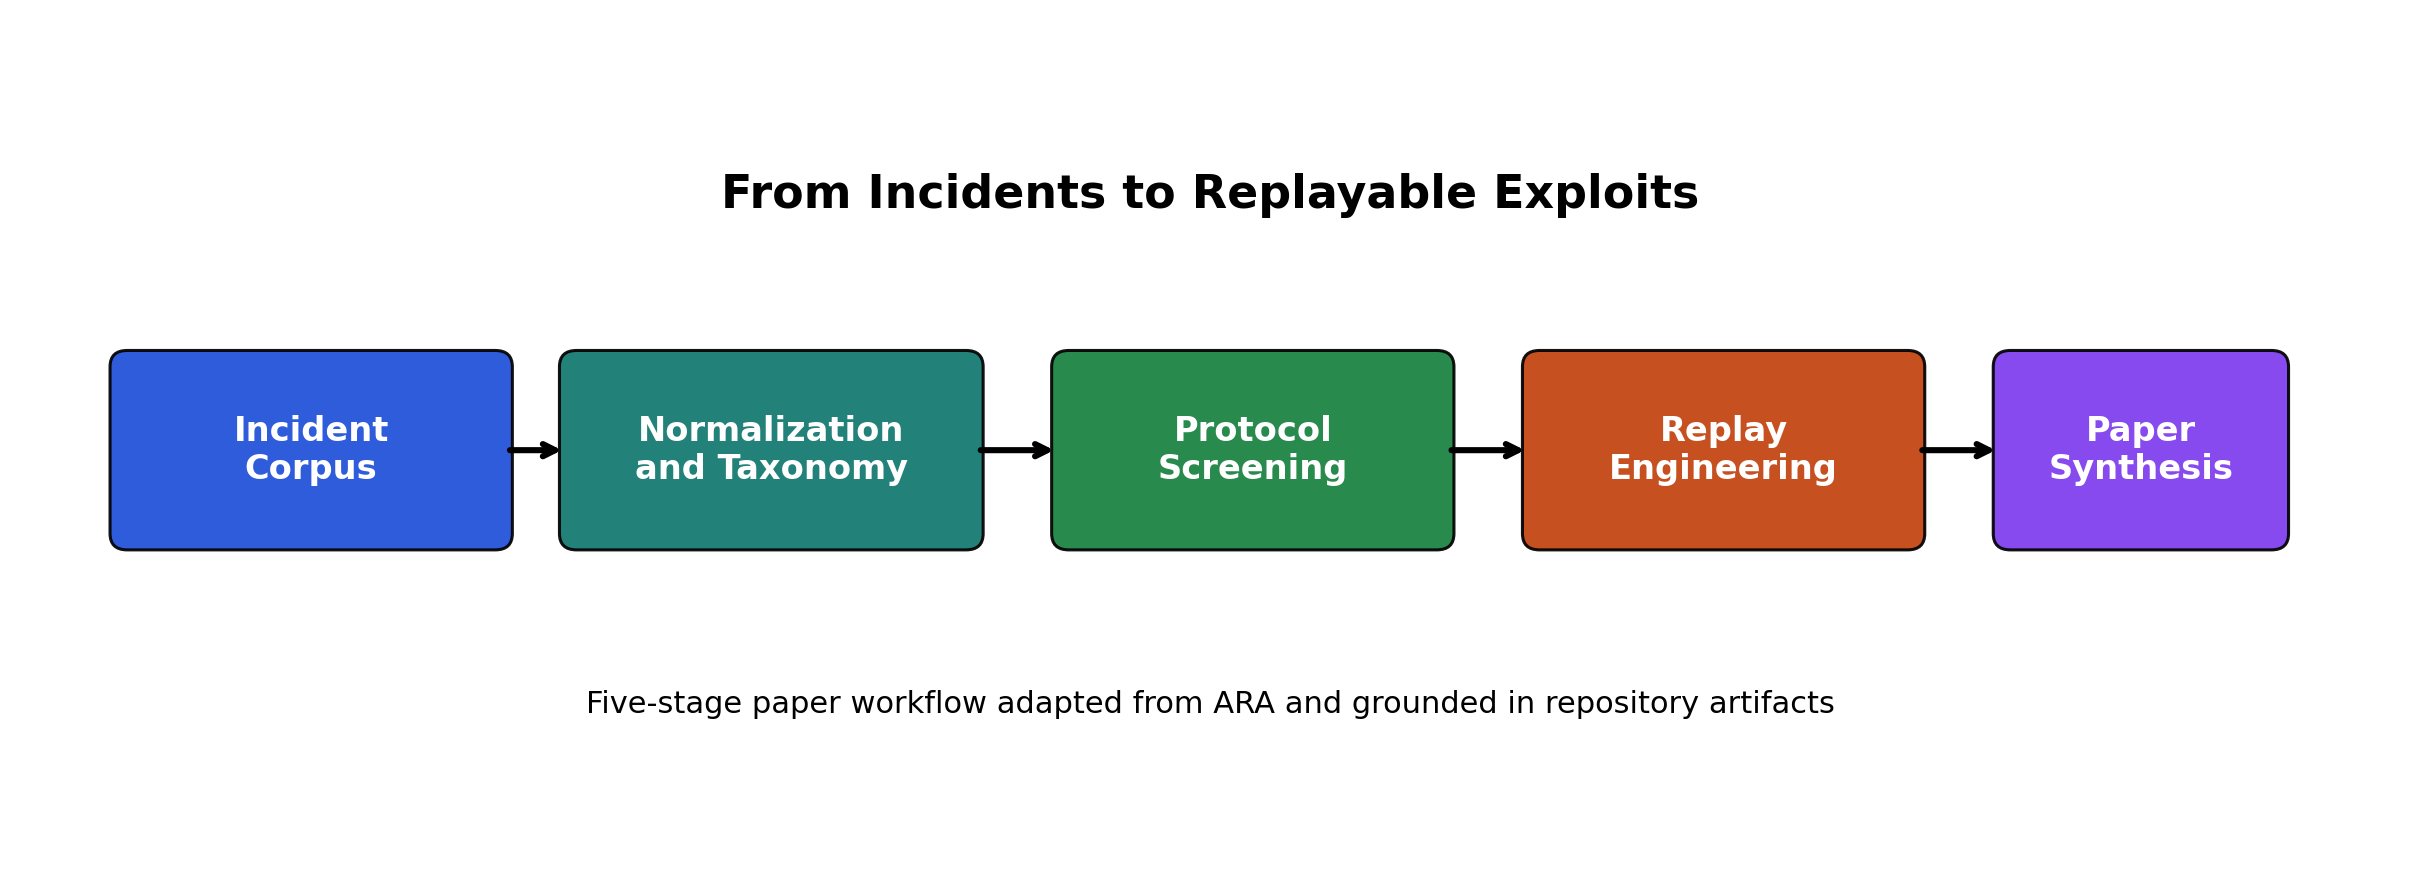
\includegraphics[width=0.98\textwidth]{research_framework.png}
\caption{Refactored paper workflow. The pipeline begins with a broad incident corpus, narrows through normalization and protocol screening, and only then promotes selected cases into replay engineering and paper claims.}
\label{fig:framework}
\end{figure}

\subsection{Evidence Layers}

The workflow is built around three evidence layers. The first is a normalized incident dataset loaded from `data/processed/incidents\_normalized\_latest.csv`, which currently contains 2{,}036 rows and 2{,}035 unique incident identifiers, of which 1{,}378 are labeled as DeFi. The second is a protocol evidence layer composed of five deep audits and a 24-protocol pure on-chain verification study. The third is a replay layer consisting of twelve shortlisted incidents, with concrete replay logic already encoded for Euler Finance, BonqDAO and AllianceBlock, and Lendf.Me.

We intentionally distinguish between \emph{confirmed exploitability}, \emph{conditional exploitability}, and \emph{replay engineering progress}. Confirmed exploitability means that the repository contains high-confidence evidence of a pure on-chain attack path under the study's threat model. Conditional exploitability means that the issue depends on downstream integrations, special market states, or missing runtime confirmation. Replay engineering progress is weaker still: it indicates whether the exploit path has been encoded as executable logic in tests, regardless of whether archive RPC validation has been completed.

\begin{table}[t]
\centering
\caption{Evidence layers and the kinds of claims they support.}
\label{tab:evidence-layers}
\begin{tabular}{p{2.2cm}p{4.0cm}p{5.3cm}}
\toprule
\textbf{Layer} & \textbf{Primary artifacts} & \textbf{Supported claims} \\
\midrule
Incident corpus & Normalized incident CSV, yearly counts, family taxonomy, loss summaries & Broad ecosystem trends, dominant categories, shortlist construction, evidence that public feeds are heterogeneous \\
Protocol evidence & Deep audits, triaged findings, 24-protocol verification report & High-confidence statements about pure on-chain exploitability under a specific threat model \\
Replay evidence & Incident cards, replay tests, fork anchors, encoded exploit logic & Mechanism-level claims about exploit preconditions and reproduction feasibility \\
\bottomrule
\end{tabular}
\end{table}

Table~\ref{tab:evidence-layers} summarizes the paper's central discipline: every claim must be attached to the layer that actually supports it. This prevents a common failure mode in security writing, where scanner findings are discussed as if they were reproduced exploits or where incident counts are discussed as if they were code-level proof.

\subsection{Scoring and Derived Metrics}

Replay work is prioritized using a pragmatic scoring rule rather than a claim of theoretical severity. For an incident $i$, we define a replayability prioritization score as
\[
S(i) = \alpha_f F(i) + \alpha_l \log(1 + L(i)) + \alpha_r R(i) + \alpha_c C(i),
\]
where $F(i)$ weights historically replayable families such as oracle manipulation, flash-loan-assisted logic abuse, and reentrancy; $L(i)$ is the reported loss in U.S. dollars; $R(i)$ indicates whether a public exploit path or post-mortem exists; and $C(i)$ represents chain and contract identifiability. This score is used operationally for shortlist construction, not as a normative security metric.

For the paper, two aggregate metrics are more important. The first is replay conversion,
\[
\mathrm{ReplayConversion} = \frac{N_{\mathrm{replay\ logic}}}{N_{\mathrm{shortlisted}}},
\]
which measures how many shortlisted incidents have already been turned into concrete replay logic. The second is protocol exposure ratio,
\[
\mathrm{ExposureRatio} = \frac{N_{\mathrm{conditional}} + N_{\mathrm{confirmed}}}{N_{\mathrm{verified}}},
\]
which measures how much of the verified protocol set remains exposed to either direct or integration-dependent pure on-chain attack paths. In the current artifact set, these values are $3/12 = 0.25$ and $4/24 \approx 0.167$, respectively.

\subsection{Threat Model and Confidence Boundaries}

The protocol-study layer uses a deliberately narrow threat model. An attack is treated as pure on-chain only if it can be executed in a single transaction or a short block window without relying on external compromise, extraordinary governance capture, or unrealistic market conditions. This choice biases the study toward precision rather than recall. It undercounts some real incidents, but it avoids conflating every observed loss with directly replayable contract exploitability. The replay layer inherits the same discipline: a scaffold or encoded exploit path is not described as fully verified unless archive RPC execution has actually succeeded.

\section{Experiments and Results}
\label{sec:experiments}

\subsection{Corpus-Level Results}

The normalized corpus provides the broadest evidentiary layer in the repository. Table~\ref{tab:dataset-summary} summarizes the headline numbers. Two observations matter immediately. First, the corpus is large enough to support trend and taxonomy analysis rather than anecdotal reasoning. Second, it remains heterogeneous even after normalization. Approximately two-thirds of all incidents are labeled as DeFi, which means a non-trivial fraction of the broader archive still falls outside the paper's focus and must be filtered out before any exploitability claim is made.

\begin{table}[t]
\centering
\caption{Dataset and study summary derived from repository artifacts.}
\label{tab:dataset-summary}
\begin{tabular}{lr}
\toprule
\textbf{Metric} & \textbf{Value} \\
\midrule
Total normalized incidents & 2{,}036 \\
Unique incident identifiers & 2{,}035 \\
DeFi-labeled incidents & 1{,}378 \\
DeFi share of full corpus & 67.68\% \\
Loss parsing coverage within DeFi subset & 68.36\% \\
Deep-audited protocols & 5 \\
Protocols in pure on-chain verification study & 24 \\
Shortlisted replay incidents & 12 \\
Replay cases with concrete logic & 3 \\
\bottomrule
\end{tabular}
\end{table}

Figure~\ref{fig:yearly-incidents} shows the yearly count of DeFi-labeled incidents in the normalized corpus. The curve rises steeply through 2021, peaks in the 2022--2023 period, and then declines in the partial 2025--2026 window. This trend should not be read as a direct measure of protocol insecurity. It also reflects reporting intensity, ecosystem expansion, and dataset timing. Still, it establishes that the corpus is large enough to justify a workflow that prioritizes filtering and mechanism identification over one-off exploit storytelling.

\begin{figure}[t]
\centering
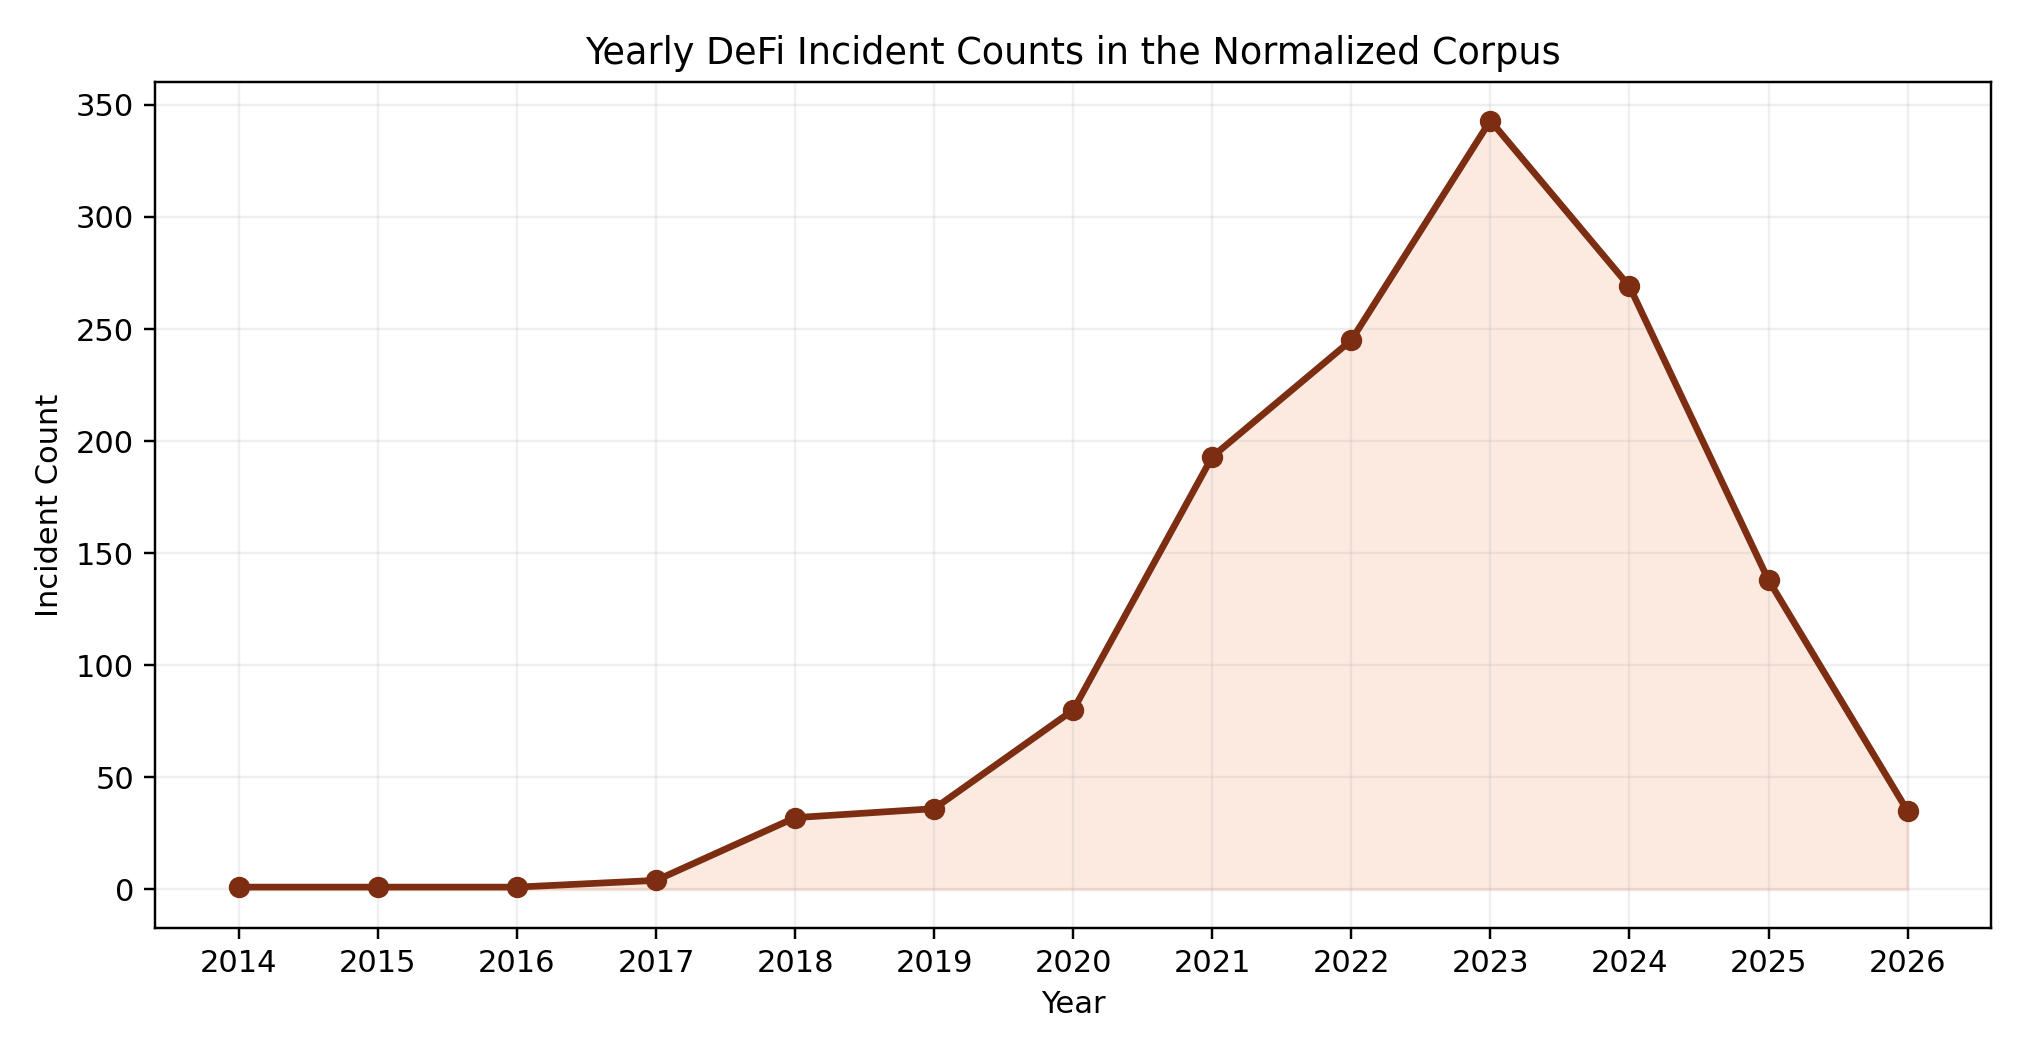
\includegraphics[width=0.93\textwidth]{yearly_defi_incidents.png}
\caption{Yearly DeFi incident counts in the normalized corpus. The trend motivates broad corpus construction but does not by itself imply replayable exploitability.}
\label{fig:yearly-incidents}
\end{figure}

Attack-family counts tell a more useful story than yearly volume. Figure~\ref{fig:family-dist} shows that the normalized DeFi subset is dominated by the \texttt{other} bucket, followed by contract bugs, flash-loan incidents, account compromise, bridge-message abuse, social engineering, and oracle manipulation. The size of the \texttt{other} bucket is itself an important result: public archives remain semantically noisy even after normalization, and any paper that translates those counts directly into exploit conclusions will overstate the prevalence of replayable smart-contract failures.

\begin{figure}[t]
\centering
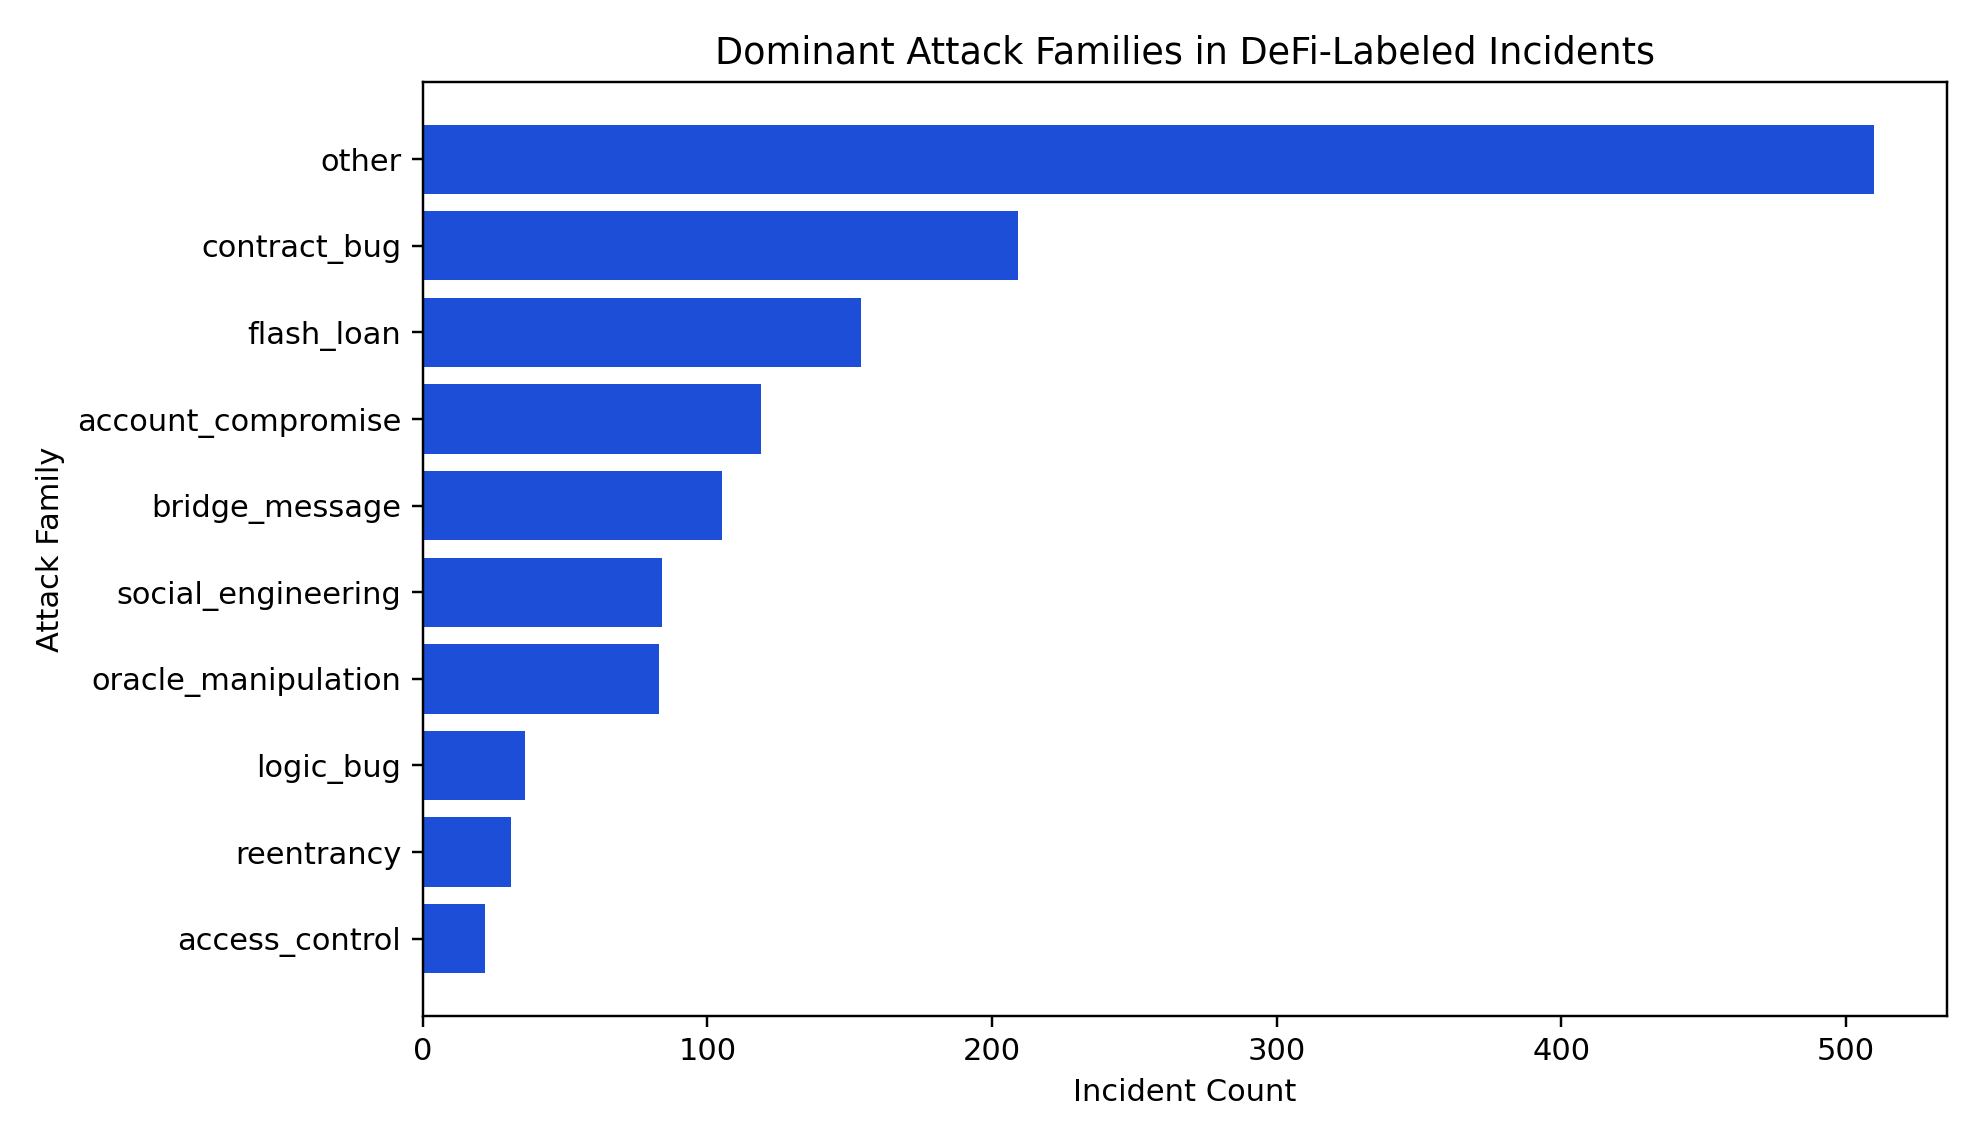
\includegraphics[width=0.93\textwidth]{incident_family_distribution.png}
\caption{Dominant attack families in the DeFi-labeled corpus. The large residual \texttt{other} category shows why incident counts cannot be treated as a clean exploitability proxy.}
\label{fig:family-dist}
\end{figure}

Loss statistics reinforce the same point. Within the DeFi-labeled subset, the median parsed loss is approximately \$891{,}000, while the top twenty incidents account for roughly \$17.26B in aggregate loss. Yet the appendix shows that many of the largest entries in the dataset fall into broad categories such as \texttt{other} or \texttt{supply\_chain}. This is precisely why the paper separates incident magnitude from replayability. A high-loss event is important evidence for ecosystem risk, but it is not automatically evidence of a replayable pure on-chain contract exploit.

\subsection{Protocol Evidence}

The repository contains two complementary protocol-level datasets. The first consists of five deep audits on Lido, Aave, Uniswap, Curve, and Compound. The second is a 24-protocol pure on-chain verification study that asks a narrower question: which major protocols still expose single-transaction or short-window exploitability under a strict threat model? Figure~\ref{fig:audit-findings} summarizes the manually triaged findings from the audit layer. The 87 findings include 5 critical, 16 high, 42 medium, and 24 low or informational issues. This distribution is useful because it demonstrates that code-level weakness density and replayable exploitability are not identical. Mature protocols still expose many hardening opportunities even when direct pure on-chain exploit paths are scarce.

\begin{figure}[t]
\centering
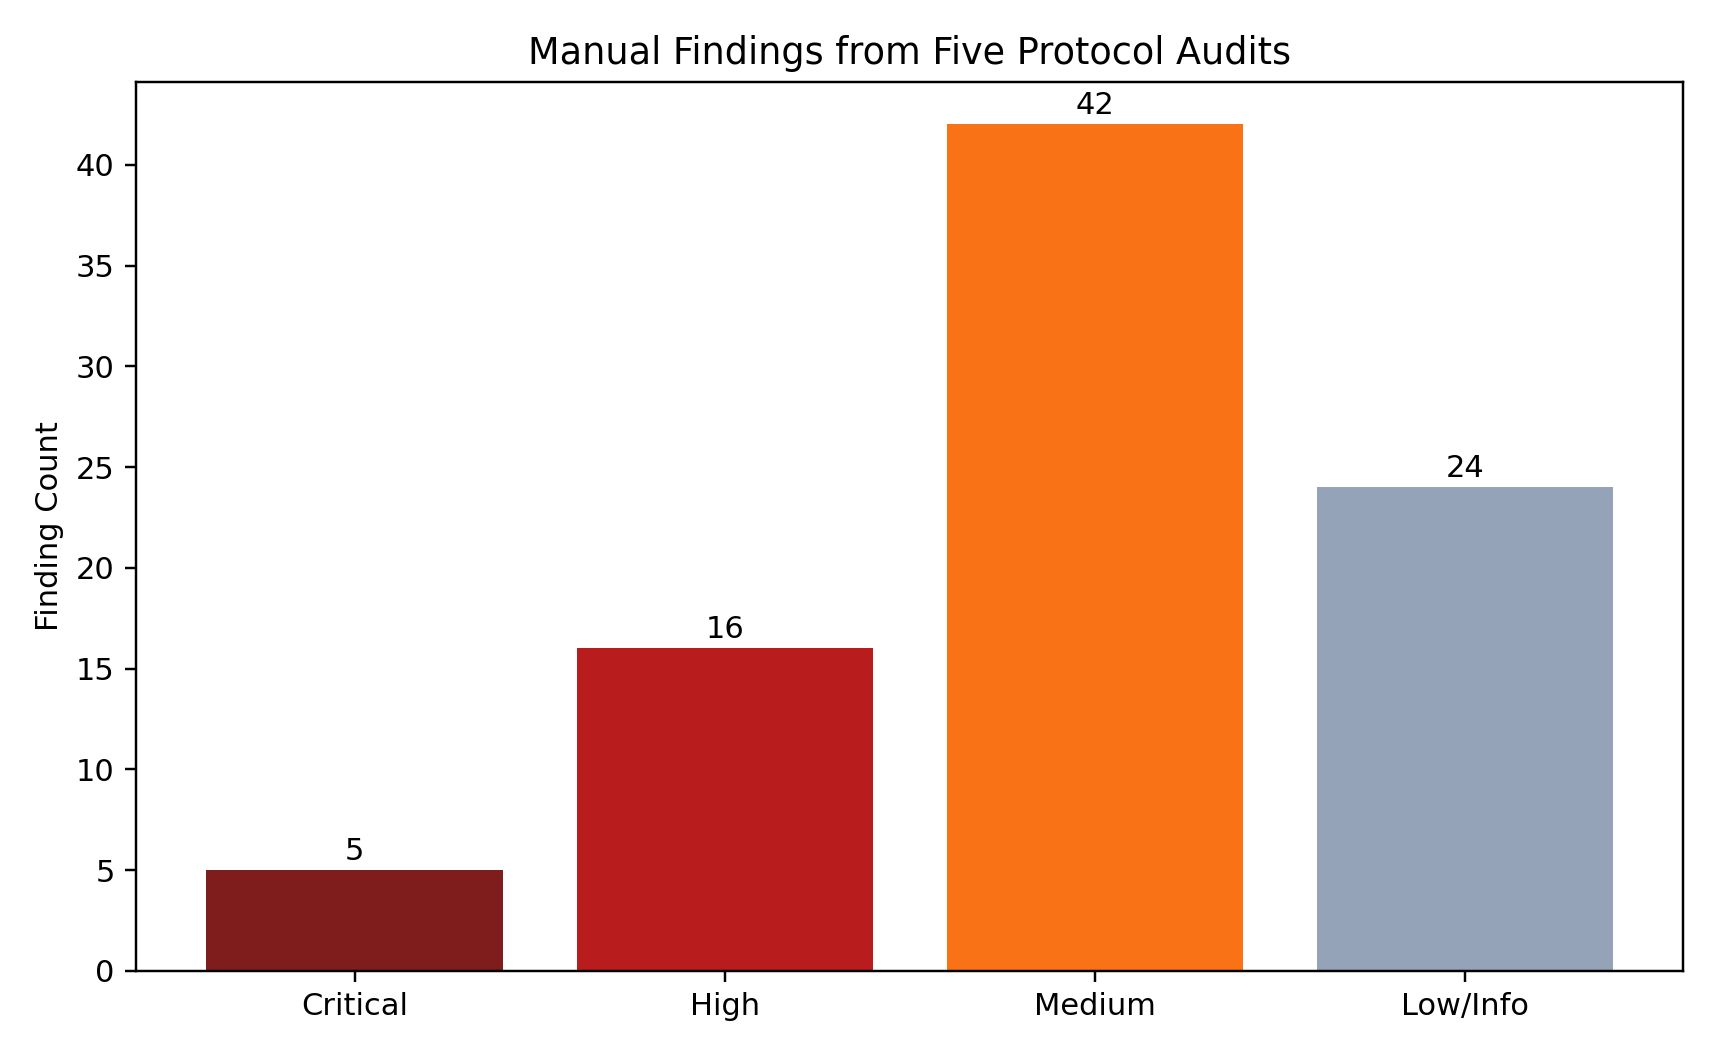
\includegraphics[width=0.80\textwidth]{audit_findings.png}
\caption{Manually triaged findings across the five deep protocol audits. Scanner output was much larger, but paper claims are based on the triaged set.}
\label{fig:audit-findings}
\end{figure}

The 24-protocol verification study yields an even sharper conclusion. As shown in Figure~\ref{fig:protocol-verdicts}, 20 protocols were judged safe under the study's pure on-chain threat model, 3 were conditional or integration-dependent, and only 1 was confirmed exploitable with high confidence. Table~\ref{tab:protocol-outcomes} makes these categories explicit. The confirmed case is Morpho Blue, where the repository contains an already validated malicious-oracle market proof of concept. The conditional set consists of Pendle, Curve, and BENQI, each of which exposes a real mechanism family but still depends on downstream integrations, empty-market states, or runtime constraints before it becomes a clean exploit.

\begin{figure}[t]
\centering
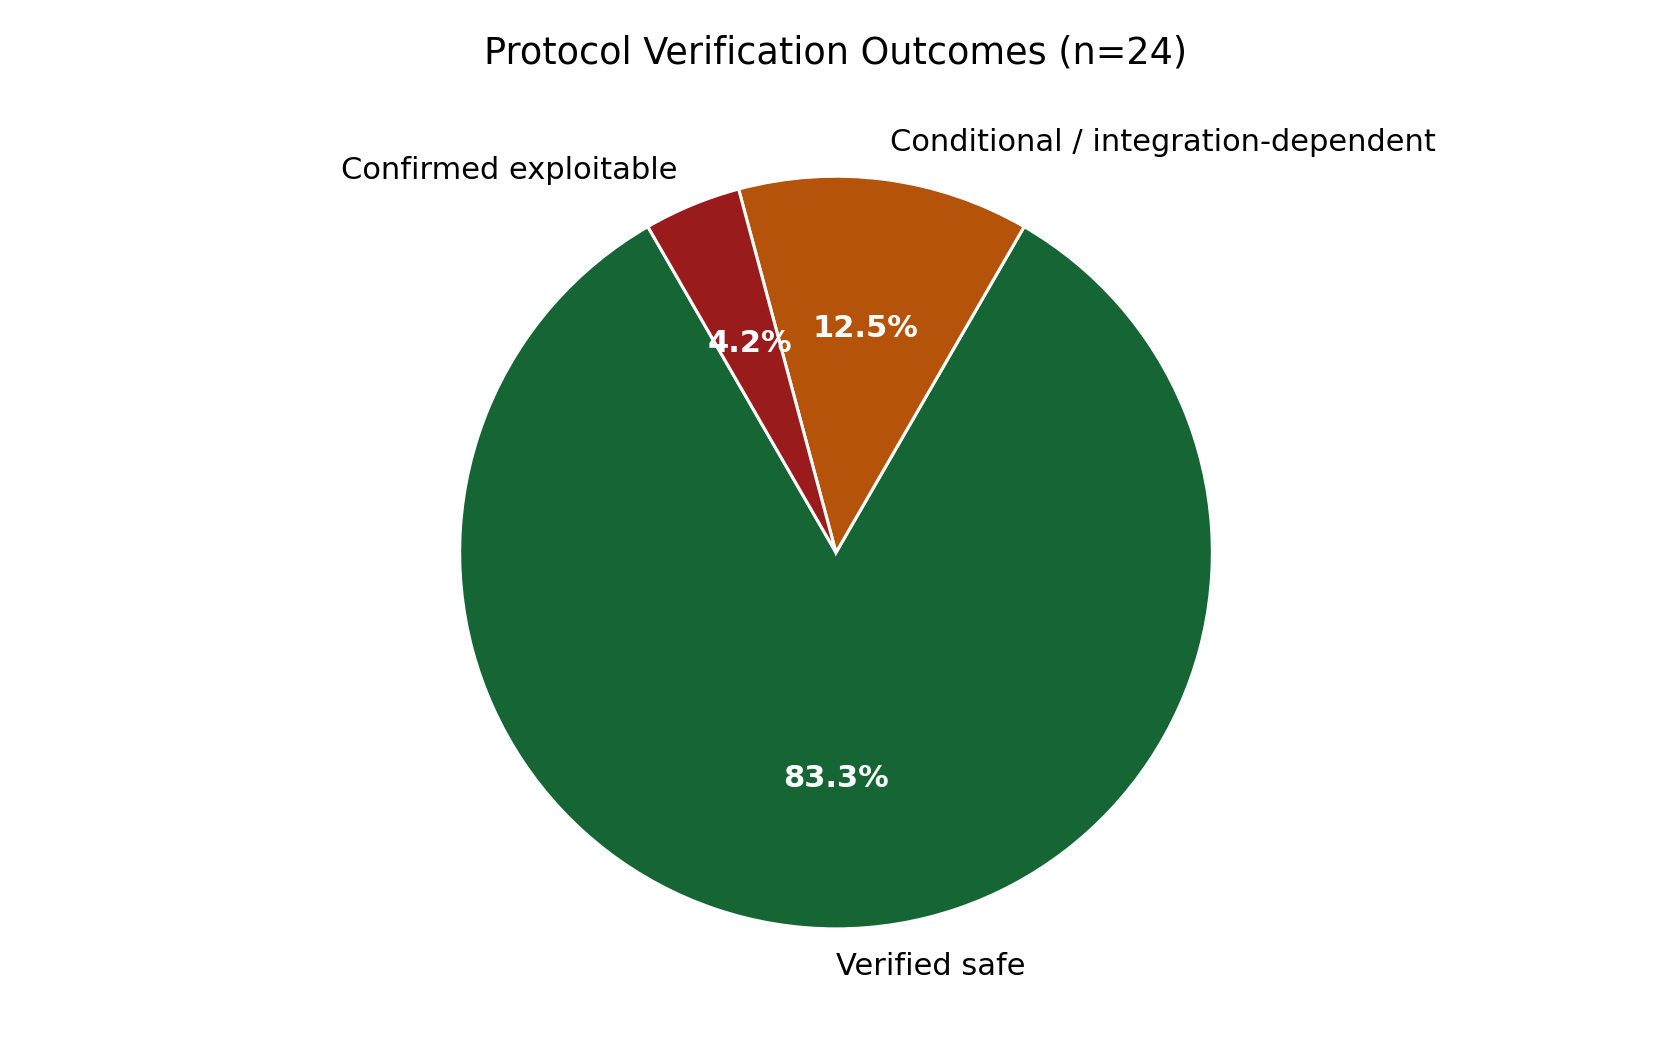
\includegraphics[width=0.74\textwidth]{protocol_verdicts.png}
\caption{Outcome categories from the 24-protocol pure on-chain verification study. The high-confidence exploitable set is materially smaller than a naive reading of the incident corpus would suggest.}
\label{fig:protocol-verdicts}
\end{figure}

\begin{table}[t]
\centering
\caption{Protocol-study outcomes under the repository's pure on-chain threat model.}
\label{tab:protocol-outcomes}
\begin{tabular}{lp{7.1cm}r}
\toprule
\textbf{Verdict} & \textbf{Interpretation} & \textbf{Count} \\
\midrule
Verified safe & No pure on-chain exploit path identified under the study assumptions & 20 \\
Conditional / integration-dependent & Attack surface exists, but exploitation depends on downstream integration, market state, or additional runtime assumptions & 3 \\
Confirmed exploitable & High-confidence pure on-chain exploit path supported by repository artifacts & 1 \\
\bottomrule
\end{tabular}
\end{table}

The protocol evidence therefore corrects a common intuition. Broad incident feeds make DeFi appear uniformly fragile, whereas protocol-level verification shows concentration: a small number of mechanism families continue to matter, but many high-TVL systems are protected by strong oracle design, constrained architecture, hardened governance, or simply the absence of a direct price-dependent lending path. The result is consistent with the intuition behind robust external price feeds such as Chainlink \citep{chainlinkDocs}, but our contribution is methodological rather than promotional: the repository demonstrates how to convert that intuition into explicit outcome categories.

Expressed as ratios, the result is even clearer. The protocol exposure ratio is approximately $4/24 = 16.7\%$ if conditional and confirmed cases are grouped together, and only $1/24 = 4.2\%$ if the threshold is raised to high-confidence confirmed exploitability. Those two values provide a practical upper and lower bound for how aggressively the current artifact set should be interpreted.

\subsection{Replay Batch Results}

Replay engineering is the final and narrowest evidence layer. The current batch contains twelve shortlisted incidents selected by loss magnitude, exploit-family relevance, and public reproducibility signals. Of those twelve, concrete replay logic has been implemented for three incidents: Euler Finance, BonqDAO and AllianceBlock, and Lendf.Me. Figure~\ref{fig:replay-cases} places those cases alongside UwU Lend, which remains shortlisted but deferred because the exploit path is materially larger and requires a dedicated pass.

\begin{figure}[t]
\centering
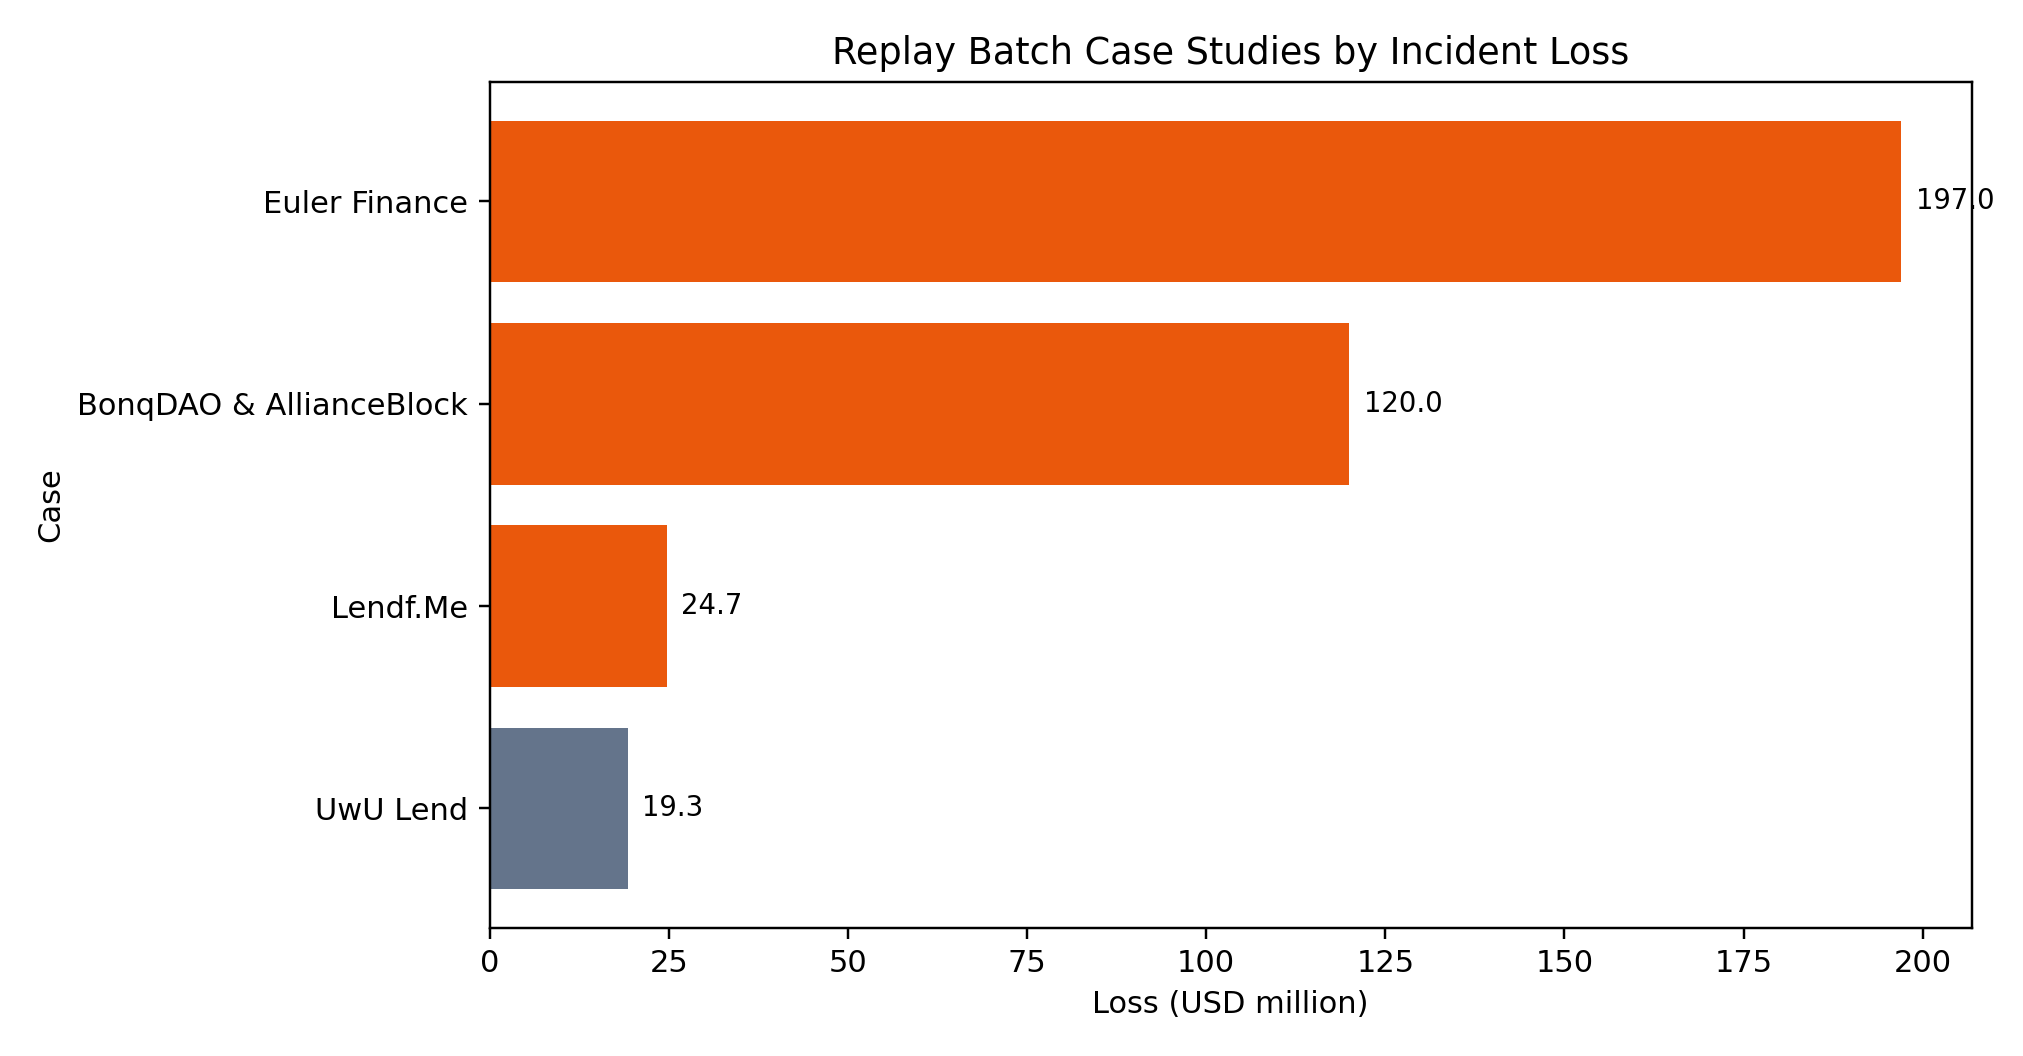
\includegraphics[width=0.93\textwidth]{replay_cases.png}
\caption{Replay batch case studies by reported loss. Orange bars indicate incidents with concrete replay logic already encoded in Foundry tests.}
\label{fig:replay-cases}
\end{figure}

\begin{table}[t]
\centering
\caption{Status of the principal replay case studies in the current paper.}
\label{tab:replay-cases}
\begin{adjustbox}{max width=\textwidth}
\begin{tabular}{llllr}
\toprule
\textbf{Case} & \textbf{Family} & \textbf{Reported loss} & \textbf{Status} & \textbf{Fork-verified} \\
\midrule
Euler Finance & Flash-loan-assisted logic abuse & \$197.0M & Logic implemented & No \\
BonqDAO \& AllianceBlock & Oracle manipulation & \$120.0M & Logic implemented & No \\
Lendf.Me & Reentrancy & \$24.7M & Logic implemented & No \\
UwU Lend & Oracle manipulation & \$19.3M & Deferred shortlist & No \\
\bottomrule
\end{tabular}
\end{adjustbox}
\end{table}

These cases are useful precisely because they represent different exploit families. Euler is a flash-loan-assisted liquidation and donation path with logic-level amplification, consistent with post-mortem analyses of the incident \citep{eulerPostmortem}. BonqDAO demonstrates how a manipulated reporting path can collapse collateral assumptions and enable outsized borrowing \citep{bonqIncident}. Lendf.Me remains the canonical callback-driven reentrancy case in which ERC777 token hooks violate assumptions about call order and state finality \citep{lendfmeIncident}. Together, the three cases support a narrower but stronger claim than the incident corpus alone: replayable exploitability in the repository clusters around a small set of mechanism families with well-understood control-flow or oracle preconditions.

The replay conversion rate is currently $3/12 = 25\%$. This number should not be interpreted as a failure. It is evidence that exploit reproduction is the most demanding stage in the workflow. Some incidents lack clean public exploit paths. Some depend on archive RPC state that is unavailable in the current shell configuration. Others, like UwU Lend, are multi-stage enough that forcing them into the batch would reduce correctness. A stronger paper is built by marking those boundaries explicitly rather than pretending that every high-loss incident is equally replayable.

\section{Discussion}
\label{sec:discussion}

The results support a disciplined reinterpretation of DeFi security evidence. The incident layer says that DeFi losses are numerous, recurrent, and diverse. The protocol layer says that pure on-chain exploitability among major protocols is much narrower. The replay layer says that even historically important incidents do not all translate cleanly into executable proofs without substantial engineering and runtime context. The contribution of the workflow is therefore epistemic as much as empirical: it forces each claim to be attached to the evidence layer that actually supports it.

Three mechanism families dominate the current artifact set. Oracle manipulation remains the clearest bridge between protocol design assumptions and replayable exploitation, especially when external price-reporting paths or thin-liquidity dependencies interact with permissive borrowing logic. Flash-loan-assisted logic abuse remains important because it converts otherwise awkward state transitions into atomic capital-efficient strategies. Reentrancy remains relevant not because every protocol is equally vulnerable, but because callback semantics and external control flow still create sharp discontinuities in otherwise mature systems. These families are consistent with prior DeFi security literature \citep{qin2021attacking,zhou2023sok}, but the repository adds concrete workflow scaffolding around them.

The audit and verification layers also suggest a practical distinction between \emph{security debt} and \emph{replayable exploitability}. A mature protocol may still accumulate dozens of medium-severity hardening issues or architectural concerns without exposing a high-confidence pure on-chain exploit path. This is visible in the five deep audits, where 87 manually triaged findings coexist with a protocol-verification result in which only one out of 24 major protocols is classified as confirmed exploitable. Research papers that ignore this distinction risk confusing engineering debt with imminent exploitability. Conversely, a workflow that only studies confirmed exploits may ignore the long tail of design weaknesses that shape future incidents.

The main limitation of the present paper is that the replay layer is still incomplete. The three principal replay cases have concrete logic encoded, but archive RPC validation has not been completed in the current environment. The protocol-verification layer also contains conditional cases whose exploitability depends on downstream integrations or edge-case market conditions. These limits do not invalidate the paper's argument; they define its scope. The paper is strongest as a methodology and intermediate empirical study, not yet as a definitive census of fully reproduced DeFi exploits.

That limitation points directly to the next phase of work. The repository should expand the replay suite from three implemented cases to at least five or eight archive-validated cases spanning oracle manipulation, reentrancy, logic abuse, and governance-assisted paths. It should also improve linkage between incident cards, protocol studies, and replay prerequisites so that each paper claim can be traced to a stable artifact. The refactored writing system created here is intended to make that next step cheaper, because it separates experiment generation, paper drafting, and revision rather than collapsing everything into a single ad hoc document.

\section{Threats to Validity}
\label{sec:threats}

\paragraph{Construct validity.}
The incident taxonomy is normalized from a public archive rather than derived from a single canonical benchmark. This creates unavoidable label noise, especially for records in which the public writeup mixes direct protocol failure with ancillary compromise or vague root-cause descriptions. We mitigate this by treating the incident corpus as a screening layer rather than final exploit evidence. Even so, the residual \texttt{other} category remains large, and this limits any fine-grained statistical claim about exact family prevalence.

\paragraph{Internal validity.}
The protocol-verification results rely on repository reports that already embed analyst judgment about exploitability under a narrow pure on-chain threat model. That judgment is deliberate, but it means the study favors precision over recall. Some incidents that were real in practice may be excluded because they required off-chain compromise, exceptional governance leverage, or market conditions not allowed by the study. Our conclusions should therefore be read as claims about replayable pure on-chain exploitability, not about total ecosystem risk.

\paragraph{External validity.}
The repository covers a non-trivial but still bounded protocol set. Five protocols received deep audits and twenty-four protocols were included in the pure on-chain verification study. These protocols are meaningful because they include major lending, AMM, and staking systems, but they do not represent every DeFi design. Results may not generalize cleanly to long-tail deployments, bespoke bridge architectures, or newly deployed protocols with immature code and low liquidity.

\paragraph{Artifact validity.}
Replay engineering remains an intermediate result rather than a final artifact evaluation. Three replay cases contain concrete logic in Foundry tests, but archive RPC execution was not completed in the present shell configuration. This matters because reproduction difficulty is part of the paper's argument. The artifact set can already support methodological conclusions, but a stronger paper will require archive-validated execution logs for at least a subset of the replay cases.

\section{Artifact Availability and Reproducibility}
\label{sec:artifact}

The repository now exposes the paper workflow as a first-class artifact. The \texttt{idea/} directory records research questions and scope controls. The \texttt{exp/} directory contains the script that regenerates all current paper tables and figures from repository data, plus the derived CSV results used by the draft. The \texttt{writing/} directory contains a blueprint, sectioned \LaTeX{} sources, bibliography, and generated figures. The \texttt{revision/} directory records the weaknesses of the previous draft and the concrete changes made in this refactor. The \texttt{build/} directory exports the compiled PDF and build log.

Reproducing the current paper requires two commands from the paper root: first run the artifact script to regenerate result tables and figures, then run the PDF build script. Because the current draft relies only on local repository data and the already-generated bibliography, this workflow is deterministic under the existing environment. Replay validation is deliberately separated from paper building. That separation keeps the writing pipeline reproducible even when archive RPC credentials are absent, while also making clear that exploit replay claims remain bounded by the available runtime evidence.

The repository now also includes a dedicated replay-validation helper script, \texttt{exp/scripts/validate\_replays.sh}, which executes the current replay cases when archive-capable \texttt{ETH\_RPC\_URL} and \texttt{POLYGON\_RPC\_URL} variables are available. On April 1, 2026, we attempted to use several public unauthenticated endpoints for this purpose. Those attempts did not produce archive-valid forks: Ethereum endpoints failed with either uninitialized fork creation or missing historical state, and the tested Polygon endpoint failed because the required historical state was unavailable. We therefore treat the current replay layer as \emph{implemented but not archive-validated}, and we record that status as an observed infrastructure constraint rather than an unexamined omission.

\section{Conclusion}
\label{sec:conclusion}

This paper reorganizes the repository's security work into a research pipeline that begins with public incidents and ends with replay-oriented exploit claims. The central empirical result is straightforward: raw incident volume is much broader than confirmed pure on-chain exploitability. Within the current artifact set, the normalized corpus contains 1{,}378 DeFi-labeled incidents, but the 24-protocol verification study identifies only one high-confidence confirmed pure on-chain exploit path and three additional conditional cases. Replay engineering narrows the lens further, with concrete logic currently implemented for three representative historical exploits.

The paper's stronger contribution is methodological. By separating incident evidence, protocol evidence, and replay evidence, the refactored workflow makes it easier to write papers that are simultaneously richer and more disciplined. It encourages stronger claims where the evidence is strong and more restrained language where the repository still contains only a scaffold, a shortlist, or a conditional finding. That is a better fit for DeFi security research than either a flat incident catalog or a scanner-driven vulnerability count.

The immediate next milestone is to convert the replay layer from implemented logic into archive-validated results. Once that happens for a broader set of cases, the same paper system can support a substantially stronger version of this study with deeper appendices, more complete case tables, and sharper comparative claims. In that sense, the present draft should be read as a credible research baseline: its main value is that it makes the next increment of evidence accumulation straightforward rather than ad hoc.

\appendix
\section{Supplementary Tables}
\label{sec:appendix}

\begin{table}[ht]
\centering
\caption{Top-loss entries in the DeFi-labeled subset. The table illustrates why incident magnitude alone is a poor proxy for replayable contract exploitability.}
\label{tab:top-losses}
\begin{adjustbox}{max width=\textwidth}
\begin{tabular}{llll}
\toprule
\textbf{Date} & \textbf{Target} & \textbf{Family} & \textbf{Loss} \\
\midrule
2019-06-29 & PlusToken & other & \$2.90B \\
2021-04-21 & Thodex & other & \$2.50B \\
2021-08-21 & BitConnect & other & \$2.00B \\
2025-02-21 & Bybit & supply\_chain & \$1.46B \\
2019-10-08 & WOTOKEN & other & \$1.11B \\
2018-04-22 & BeautyChain & other & \$1.00B \\
2016-08-03 & Bitfinex & other & \$0.90B \\
2019-04-26 & Bitfinex & other & \$0.85B \\
2020-07-10 & BitClub & other & \$0.72B \\
2021-08-10 & Poly Network & bridge\_message & \$0.61B \\
\bottomrule
\end{tabular}
\end{adjustbox}
\end{table}

\begin{table}[ht]
\centering
\caption{Replay prerequisites for the three implemented case studies.}
\label{tab:replay-prereqs}
\begin{adjustbox}{max width=\textwidth}
\begin{tabular}{llll}
\toprule
\textbf{Case} & \textbf{Chain} & \textbf{Fork anchor} & \textbf{Test file} \\
\midrule
Euler Finance & Ethereum & block 16{,}817{,}995 & \texttt{test/replay/EulerFinanceReplay.t.sol} \\
BonqDAO \& AllianceBlock & Polygon & block 38{,}792{,}977 & \texttt{test/replay/BonqDAOReplay.t.sol} \\
Lendf.Me & Ethereum & block 9{,}899{,}725 & \texttt{test/replay/LendfMeReplay.t.sol} \\
\bottomrule
\end{tabular}
\end{adjustbox}
\end{table}

\begin{table}[ht]
\centering
\caption{Observed outcomes from April 1, 2026 public RPC validation attempts.}
\label{tab:rpc-validation}
\begin{adjustbox}{max width=\textwidth}
\begin{tabular}{llll}
\toprule
\textbf{Case} & \textbf{Endpoint} & \textbf{Outcome} & \textbf{Interpretation} \\
\midrule
Lendf.Me & \texttt{eth.llamarpc.com} & Historical state unavailable & Free endpoint lacks required archive depth \\
Lendf.Me & \texttt{ethereum-rpc.publicnode.com} & Historical state unavailable & Free endpoint lacks required archive depth \\
Lendf.Me & \texttt{eth-mainnet.public.blastapi.io} & Fork not initialized & Fork creation not usable for this replay \\
BonqDAO & \texttt{polygon-bor-rpc.publicnode.com} & Historical state unavailable & Free endpoint lacks required archive depth \\
\bottomrule
\end{tabular}
\end{adjustbox}
\end{table}


\bibliography{references}
\bibliographystyle{analemma}
\end{document}
